%%%%%%%%%%%%%%%%%%%%%%%%%%%%%%%%%%%%%%%%%%%%%%%%%%%%%%%%%%%%%%%%%%%%
%%%%%%%%%%%%%%%%%%%%%%%%%%%%%%%%%%%%%%%%%%%%%%%%%%%%%%%%%%%%%%%%%%%%
%%                                                                %%
%% An example for writting your thesis using LaTeX                %%
%% Original version by Luis Costa,  changes by Perttu Puska       %%
%% Support for Swedish added 15092014                             %%
%%                                                                %%
%% This example consists of the files                             %%
%%         thesistemplate.tex (versio 2.01)                       %%
%%         opinnaytepohja.tex (versio 2.01) (for text in Finnish) %%
%%         aaltothesis.cls (versio 2.01)                          %%
%%         kuva1.eps                                              %%
%%         kuva2.eps                                              %%
%%         kuva1.pdf                                              %%
%%         kuva2.pdf                                              %%
%%                                                                %%
%%                                                                %%
%% Typeset either with                                            %%
%% latex:                                                         %%
%%             $ latex opinnaytepohja                             %%
%%             $ latex opinnaytepohja                             %%
%%                                                                %%
%%   Result is the file opinnayte.dvi, which                      %%
%%   is converted to ps format as follows:                        %%
%%                                                                %%
%%             $ dvips opinnaytepohja -o                          %%
%%                                                                %%
%%   and then to pdf as follows:                                  %%
%%                                                                %%
%%             $ ps2pdf opinnaytepohja.ps                         %%
%%                                                                %%
%% Or                                                             %%
%% pdflatex:                                                      %%
%%             $ pdflatex opinnaytepohja                          %%
%%             $ pdflatex opinnaytepohja                          %%
%%                                                                %%
%%   Result is the file opinnaytepohja.pdf                        %%
%%                                                                %%
%% Explanatory comments in this example begin with                %%
%% the characters %%, and changes that the user can make          %%
%% with the character %                                           %%
%%                                                                %%
%%%%%%%%%%%%%%%%%%%%%%%%%%%%%%%%%%%%%%%%%%%%%%%%%%%%%%%%%%%%%%%%%%%%
%%%%%%%%%%%%%%%%%%%%%%%%%%%%%%%%%%%%%%%%%%%%%%%%%%%%%%%%%%%%%%%%%%%%

%% Uncomment one of these:
%% the 1st when using pdflatex, which directly typesets your document in
%% pdf (use jpg or pdf figures), or
%% the 2nd when producing a ps file (use eps figures, don't use ps figures!).
\documentclass[english,12pt,a4paper,pdftex,elec,utf8]{aaltothesis}
%\documentclass[english,12pt,a4paper,dvips]{aaltothesis}

%% To the \documentclass above
%% specify your school: arts, biz, chem, elec, eng, sci
%% specify the character encoding scheme used by your editor: utf8, latin1

%% Use one of these if you write in Finnish (see the Finnish template):
%%
%\documentclass[finnish,12pt,a4paper,pdftex,elec,utf8]{aaltothesis}
%\documentclass[finnish,12pt,a4paper,dvips]{aaltothesis}

\usepackage{graphicx}
\graphicspath{ {images/} }
\usepackage{listings}

%% Use this if you write hard core mathematics, these are usually needed
\usepackage{amsfonts,amssymb,amsbsy}

%% Use the macros in this package to change how the hyperref package below 
%% typesets its hypertext -- hyperlink colour, font, etc. See the package
%% documentation. It also defines the \url macro, so use the package when 
%% not using the hyperref package.
%%
%\usepackage{url}

%% Use this if you want to get links and nice output. Works well with pdflatex.
\usepackage{hyperref}
\hypersetup{pdfpagemode=UseNone, pdfstartview=FitH,
  colorlinks=true,urlcolor=red,linkcolor=blue,citecolor=black,
  pdftitle={Default Title, Modify},pdfauthor={Your Name},
  pdfkeywords={Modify keywords}}


%% All that is printed on paper starts here
\begin{document}

%% Change the school field to specify your school if the automatically 
%% set name is wrong
% \university{aalto-yliopisto}
\university{aalto University}
% \school{Sähkötekniikan korkeakoulu}
\school{School of Electrical Engineering}

%% Only for B.Sc. thesis: Choose your degree programme. 
%\degreeprogram{Electronics and electrical engineering}
%%

%% ONLY FOR M.Sc. AND LICENTIATE THESIS: Specify your department,
%% professorship and professorship code. 
%%
\department{Department of Radio Science and Technology}
\professorship{Space Science and Technology}
%%

%% Valitse yksi näistä kolmesta
%%
%% Choose one of these:
%\univdegree{BSc}
\univdegree{MSc}
%\univdegree{Lic}

%% Your own name (should be self explanatory...)
\author{Juha-Matti Lukkari}

%% Your thesis title comes here and again before a possible abstract in
%% Finnish or Swedish . If the title is very long and latex does an
%% unsatisfactory job of breaking the lines, you will have to force a
%% linebreak with the \\ control character. 
%% Do not hyphenate titles.
%% 
\thesistitle{Automated functional system testing of Suomi 100 satellite}

\place{Espoo}

%% For B.Sc. thesis use the date when you present your thesis. 
%% 
%% Kandidaatintyön päivämäärä on sen esityspäivämäärä! 
\date{16.1.2015}

%% B.Sc. or M.Sc. thesis supervisor 
%% Note the "\" after the comma. This forces the following space to be 
%% a normal interword space, not the space that starts a new sentence. 
%% This is done because the fullstop isn't the end of the sentence that
%% should be followed by a slightly longer space but is to be followed
%% by a regular space.
%%
\supervisor{Prof.\ Esa Kallio} %{Prof.\ Pirjo Professori}

%% B.Sc. or M.Sc. thesis advisors(s). You can give upto two advisors in
%% this template. Check with your supervisor how many official advisors
%% you can have.
%%
%\advisor{Prof.\ Pirjo Professori}
\advisor{D.Sc.\ (Tech.) Antti Kestilä}
\advisor{D.Sc.\ (Tech.) Juha Itkonen}

%% Aalto logo: syntax:
%% \uselogo{aaltoRed|aaltoBlue|aaltoYellow|aaltoGray|aaltoGrayScale}{?|!|''}
%%
%% Logo language is set to be the same as the document language.
%% Logon kieli on sama kuin dokumentin kieli
%%
\uselogo{aaltoRed}{''}

%% Create the coverpage
%%
\makecoverpage


%% Note that when writting your master's thesis in English, place
%% the English abstract first followed by the possible Finnish abstract

%% English abstract.
%% All the information required in the abstract (your name, thesis title, etc.)
%% is used as specified above.
%% Specify keywords
%%
%% Kaikki tiivistelmässä tarvittava tieto (nimesi, työnnimi, jne.) käytetään
%% niin kuin se on yllä määritelty.
%% Avainsanat
%%
\keywords{For keywords choose concepts that are central to your thesis}
%% Abstract text
\begin{abstractpage}[english]
 Large portion of launched Cubesats have failed early on their missions. Complete lack or inadequate system level functional testing of the satellites has been thought of being one large contributor to these failures according to some research done on the statistical data available about Cubesats. This thesis investigates potential solutions to mitigating these issues by the use of free open-source automated test framework. Presenting how we can do system level testing of Cubesats and what kind of tests could be done.

  Your abstract in English. Try to keep the abstract short; approximately 
  100 words should be enough. The abstract explains your research topic, 
  the methods you have used, and the results you obtained.  
  Your abstract in English. Try to keep the abstract short; approximately 
  100 words should be enough. The abstract explains your research topic, 
  the methods you have used, and the results you obtained.  
\end{abstractpage}

%% Force a new page so that the possible English abstract starts on a new page
%%
%% Pakotetaan uusi sivu varmuuden vuoksi, jotta 
%% mahdollinen suomenkielinen ja englanninkielinen tiivistelmä
%% eivät tule vahingossakaan samalle sivulle
\newpage
%
%% Abstract in Finnish.  Delete if you don't need it. 
\thesistitle{Automatisoitu Suomi 100 satelliitin funktionaalinen systeemitestaus}
\advisor{Prof Esa Kallio}
\degreeprogram{Electronics and electrical engineering}
\department{Radiotieteen ja -tekniikan laitos}
\professorship{Avaruus tiede ja tekniikka}
%% Avainsanat
\keywords{Vastus, Resistanssi,\\ Lämpötila}
%% Tiivistelmän tekstiosa
\begin{abstractpage}[finnish]
  Tiivistelmässä on lyhyt selvitys (noin 100 sanaa)
  kirjoituksen tärkeimmästä sisällöstä: mitä ja miten on tutkittu,
  sekä mitä tuloksia on saatu. 
  Tiivistelmässä on lyhyt selvitys (noin 100 sanaa)
  kirjoituksen tärkeimmästä sisällöstä: mitä ja miten on tutkittu,
  sekä mitä tuloksia on saatu. 

  Tiivistelmässä on lyhyt selvitys (noin 100 sanaa)
  kirjoituksen tärkeimmästä sisällöstä: mitä ja miten on tutkittu,
  sekä mitä tuloksia on saatu. 
  Tiivistelmässä on lyhyt selvitys (noin 100 sanaa)
  kirjoituksen tärkeimmästä sisällöstä: mitä ja miten on tutkittu,
  sekä mitä tuloksia on saatu. 
  Tiivistelmässä on lyhyt selvitys (noin 100 sanaa)
  kirjoituksen tärkeimmästä sisällöstä: mitä ja miten on tutkittu,
  sekä mitä tuloksia on saatu. 
\end{abstractpage}

%% Force new page so that the Swedish abstract starts from a new page
\newpage
%
%% Swedish abstract. Delete if you don't need it. 
%% 
\thesistitle{Arbetets titel}
\advisor{TkD Olli Ohjaaja} %
\degreeprogram{Electronik och electroteknik}
\department{Institutionen för radiovetenskap och -teknik}%
\professorship{Kretsteori}  %
%% Abstract keywords
\keywords{Nyckelord p\aa{} svenska,\\ Temperatur}
%% Abstract text
\begin{abstractpage}[swedish]
 Sammandrag p\aa{} svenska.
 Try to keep the abstract short, approximately 
 100 words should be enough. Abstract explains your research topic, 
 the methods you have used, and the results you obtained.  
\end{abstractpage}

%% Preface
%%
%% Esipuhe 
\mysection{Preface}
%\mysection{Esipuhe}
I want to thank Professor Esa Kallio
and my instructors Antti Kestilä and Juha Itkonen for their 
good guidance.\\

\vspace{5cm}
Otaniemi, 16.1.2015

\vspace{5mm}
{\hfill Eddie E.\ A.\ Engineer \hspace{1cm}}

%% Force new page after preface
%%
%% Pakotetaan varmuuden vuoksi esipuheen jälkeinen osa
%% alkamaan uudelta sivulta
\newpage


%% Table of contents. 
\thesistableofcontents


%% Symbols and abbreviations
\mysection{Symbols and abbreviations}

\subsection*{Symbols}

\begin{tabular}{ll}
$\mathbf{B}$  & magnetic flux density  \\
$c$              & speed of light in vacuum $\approx 3\times10^8$ [m/s]\\
$\omega_{\mathrm{D}}$    & Debye frequency \\
$\omega_{\mathrm{latt}}$ & average phonon frequency of lattice \\
$\uparrow$       & electron spin direction up\\
$\downarrow$     & electron spin direction down
\end{tabular}

\subsection*{Operators}

\begin{tabular}{ll}
$\nabla \times \mathbf{A}$              & curl of vectorin $\mathbf{A}$\\
$\displaystyle\frac{\mbox{d}}{\mbox{d} t}$ & derivative with respect to 
variable $t$\\[3mm]
$\displaystyle\frac{\partial}{\partial t}$  & partial derivative with respect 
to variable $t$ \\[3mm]
$\sum_i $                       & sum over index $i$\\
$\mathbf{A} \cdot \mathbf{B}$    & dot product of vectors $\mathbf{A}$ and 
$\mathbf{B}$
\end{tabular}

\subsection*{Abbreviations}

\begin{tabular}{ll}
OBC         & On board computer \\
EPS      & Electric power system \\
BCS        & Bardeen-Cooper-Schrieffer \\ %% dash between the names
DC         & direct current \\
TEM        & transverse eletromagnetic
\end{tabular}


%% Tweaks the page numbering to meet the requirement of the thesis format:
%% Begin the pagenumbering in Arabian numerals (and leave the first page
%% of the text body empty, see \thispagestyle{empty} below).
%% Additionally, force the actual text to begin on a new page with the 
%% \clearpage command.
%% \clearpage is similar to \newpage, but it also flushes the floats (figures
%% and tables).
%% There is no need to change these
%%
\cleardoublepage
\storeinipagenumber
\pagenumbering{arabic}
\setcounter{page}{1}


%% Text body begins. Note that since the text body
%% is mostly in Finnish the majority of comments are
%% also in Finnish after this point. There is no point in explaining
%% Finnish-language specific thesis conventions in English. Someday 
%% this text will possibly be translated to English.
%%
\section{Introduction}
%\section{Introduction}

%% Ensimm\"ainen sivu tyhj\"aksi
%% 
%% Leave first page empty
\thispagestyle{empty}
\subsection{Increasing interest in space}
Since 1950s, mankind has ever increasingly started to set its foot into space. Nations, industries, businesses, militaries, universities and even private entrepreneurs have sought out to benefit from the opportunities that space offers. Great advancements have been made in technology and science to propel this endeavour even further. Examples of such leaps in techology include sending first human into space in 1957, moon landings in 1969, sending of probes into other planets in the solar system like Mars and most recenlty getting the first images of Pluto in a flyby mission in 2013. Use of space technology has also entered into household items through for example the use of the GPS satellite network in mobile phones, cars, etc. People and industries have began increasingly to be reliant on space borne technologies and devices. [sources]\par
Since the end of the 1990s new inventions have brought design and manufacturing of these technologies relatively closer to everyday people, away from the assembly sites of large nations and large organizations into laboratories run for example by university students. Advancements leading to this can be attributed to the space industry cathcing up with the advancements of electronics as well as cheap launch opportunities coming available. More concretely, development of the \textit{CubeSat} nanosatellite concept in 1999 in CalTech has in recent years brought about hundreds of new satellite developers and hundreds of new space missions based on this nanosatellite concept. \cite{Swart1, Swart2016}\par 
These satellites typically are relatively small and usually use commercial off-the-self components, yet are still capable to operate in space around Earth. Cubesats have in recent years emerged as a new viable platform for carrying out space missions. Due to their small size the launch costs are smaller and their use of COTS components makes them relatively fast and relatively cheap to design and manufacture.  Several companies have taken interest into the concept and other organizations (like US military) have shown interest into them as well. In addition, Finnish government recently passed a new law regarding space and is pursuing to create a new industry of space technology related companies in Finland [source]. The first Cubesats built in Finland in Aalto University have even created new space companies which are building their own satellites to be launched into space, like \textit{Iceye} for example  [source]. Nonetheless, usually most of these satellites have been produced by Universities and over 400 Cubesats have already been launched in total since 2000 \cite{Swart2016}. The trend seems to be so that more and more CubeSat missions are to come and they are starting to take a clear share of the space industry market.[Spaceworks] Already in 2014, approximately half of the flown space missions in that year were CubeSats. \cite{Swart2016}\par 
\subsection{Substantial proportion of failures in CubeSat missions}
Even though the CubeSat concept has rapidly created large amount of new space missions, large portion of those launched missions have ended in failure due to various reasons. Several surveys done in recent years have found a failure rate of 40 \% for new CubeSat missions. Yet, if the satellites were manufactured by teams with earlier experience in space missions, the failure rates were considerably lower. Suggestions have been made in these surveys that the missions that have failed haven't done proper functional testing on ground on a system level or that such testing has been missing completely. As an example, research done by Swartwout in 2013 into statistical data of first 100 flown Cubesats discovered that over 40 \% of Cubesat missions ended in failure. This research suggests that majority of these failures could be attributed to inadequate testing of the satellite in a flight-equivalent state on ground. It was believed that functional testing of the whole integrated satellite system has been lacking completely or done in a very limited sense. This allegation could been made at least for those missions where the satellite was never contacted from the ground station after the launch, as many of the failures in these missions were attributed to failures in system integration. Such as the solar panels not being properly connected, insufficient power generated for the transmitter, unrecoverable processor errors and so forth. \cite{Swart1, Swart2016, Swart2015, Langer}\par
Some examples of early life failures include Aalto-2 satellite, the first Finnish satellite flown in space [source]. Though the concept of Cubesats shows promise, there are still some challenges for the concept to become a truly reliable alternative approach for scientific and commercial missions alike as opposed to the more traditional time and resources consuming approaches in space mission development \cite{Swart1}.\par 
\subsection{Suomi100 Cubesat} 
The satellite involved in our research is called \textit{Suomi100}. Which is a one unit Cubesat. An artistic presentation can be seen in Figure \ref{s100intro} below.
\begin{centering}
\begin{figure}[h!]
\includegraphics[scale=0.2]{s100_orbit}
\caption{Depiction of Suomi100 satellite in space.}
\label{s100intro}
\end{figure} 
\end{centering}
\subsection{Research purpose and goals}
The aim of this thesis is to investigate how could we carry out
functional system testing of Cubesats. Further, we wish to automate the testing and to do it systematically, just as the verification tests for example for mechanical stress are done systematically. For example the vibrational tests for our \textit{Suomi100} was done in VTT by automatically controlled vibration machine, where a user enters the testing program for different axes. So too it would be preferable that the functional system tests could be done automatically in a systematic manner.\par 
This thesis will provide a means to do automated functional system testing on the Suomi100 satellite and a template (joku muu sana?) for other future Cubesat missions to use when developing this form of testing for their own missions. Including a generic python library for use with Robot Framework and examples of test setups and test suites. 
\subsection{Main questions and problems}
The main problem is the unreliability of Cubesats and could we improve their reliability by carrying out functional system tests and by running the satellite in a functionally flight-equivalent state? Could we detect unrecoverable failures in the satellite operation and could we verify that the satellite meets out its functional requirements?
\subsection{Outlining the scope of research}
We wish to study the use of one industry-proven automated acceptance framework to carry out the automated functional testing on Suomi100 and to investigate the use of industry-proven testing philosophies and methodologies into functional system testing with the satellite.\par
As a "day in the life of the satellite" was pointed to be necessary to be tested, we attempt to some degree simulate the environment related to the functional operations of the satellite.  Yet, all within the resources of an university led project with relatively small funds.
%% Esimerkki luettelosta. Lyhyt ajatusviiva on k\"ayt\"oss\"a
%% luettelossa, ja se on pituudeltaan
%% en dash. Merkit\"a\"an latex-koodissa --. 


\begin{itemize}
\item[--] Research question: How can we do functional system testing on Cubesats? Can we improve the reliability of our satellite by doing these kind of tests on it?
\item[--]Failures in space industry history
\item[--]Suomi100 satellite mission
\item[--]Doing test automation for Suomi100 satellite

\item[--]Test the recoveries from faults thoroughly
\item[--]As pointed out from others research, test situation where power comes only from the solar panels and use the link to send commands to the satellite. And this for long enough. All the basic operations. Take picture, measure radio data, send telemetry.
\item[--]Robot framework. Fits to the COTS approach of Cubesats. Has been widely used already and is modular. Is open-source.
\item[--]Automated testing was considered part of "extreme programming" during 90s, which could explain why the more developed testing methods are not so widely used.
\end{itemize}


%% Opinn\"aytteess\"a jokainen osa alkaa uudelta sivulta, joten \clearpage
%%
%% In a thesis, every section starts a new page, hence \clearpage
\clearpage

\section{Background}
%\section{Aikaisempi tutkimus}
\subsection{Statistics of Cubesat failures}
Something general about cubesats. Number of launched CubeSats has increased quite dramatically over the past few years. Already in 2013 more than half of the launched missions were secondary payloads and clear majority of them were CubeSats. 
\subsubsection{Failure rates of CubeSats}
Over 400 Cubesats have flown as of 2017 \cite{Swart2016}. Few studies in recent years have been carried out to investigate the statistics of flown Cubesat missions. These studies looked for the percentage of failed missions and which subsystems contributed to each failure. Out of these failures, the amount of dead on arrival (DOA) missions where the satellite was never contacted from space were also identified. Most active contributor to this topic has been Michael Swartwout and the representation of statistics of CubeSat failures in this thesis is mainly based on his work, as not too many papers have yet been published regarding this issue.\par 
A study titled \textit{The First One hundred CubeSats: A Statistical Look} and published in 2013 was one of the first papers to analyze the statistical data of flown CubeSats. Out of the first 100 CubeSat missions investigated between years 2000-2012, a total of 34 had failed. Out of these failures, third were never contacted after they were released into space (DOA cases). Figure \ref{100first} shows the clear amount of failed missions out of the first 100 flown CubeSats. \cite{Swart1} \par
\begin{figure}[h!]
\includegraphics[scale=0.3]{2013_failures}
\caption{Statistics of first 100 flown CubeSats. \cite{Swart1}}
\label{100first}
\end{figure} 
Same author has been continuing yearly to publish papers about the statistics of CubeSat failures, as new missions are flown each year \cite{Swart2016, Swart2015}. In these papers he has included statistics about other secondary payloads as well, though majority of secondary payloads have been CubeSats. A study published in 2016 titled \textit{Secondary Spacecraft in 2016:
Why Some Succeed (And Too Many Do Not)} identified out of all CubeSats flown between 2000-2015 that reached orbit 21 \% DOA cases and 9.8 \% cases where the spacecraft was lost early in its life, meaning that communication with the satellite was established but no primary operations could have been executed. When breaking down the statistics to categories based on the type of satellite and mission developer (new University teams, traditional contractors, experienced University and government teams, constellations), it was found that for the new University teams flying their first satellite, the failure rates were as follows: 44.1 \% DOA, 16.2 \% early loss and 16.2 \% mission success. On the other hand, for the CubeSats built by traditional contractors with established practices for integration and testing the numbers were: 6.3 \% DOA and 6.3 \% early loss. On the other hand, when the new University teams educated by their first failure flew their second satellite, the rates for DOA failures halved. \cite{Swart2016, Swart2015}\par 
Below Figure \ref{hobbyistflown2015pic} shows the statistics of failures for CubeSats between 2000-2015 flown by new University teams sending their first satellite, excluding those missions where the satellite was lost due to launch failure.\par 
\begin{figure}[h!]
\includegraphics[scale=0.5]{hobbyistflown2015}
\caption{Statistics for CubeSats flown between 2000-2015 that were constructed by University teams without prior experience for satellite construction. \cite{Swart2016}}
\label{hobbyistflown2015pic}
\end{figure} 
For contrast, same statistics for CubeSats built by traditional contractors is shown in figure \ref{tradiotionalflown2015pic} below. \par
\begin{figure}[h!]
\includegraphics[scale=0.5]{traditionalflown2015}
\caption{Statistics for CubeSats flown between 2000-2015 that were constructed by traditional contractors with extensive experience of satellite construction. \cite{Swart2016}}
\label{tradiotionalflown2015pic}
\end{figure} 
\subsubsection{Contribution of different subsystems to satellite failures}
Some study has been carried out by Swartwout in one of the aforementioned papers to investigate the contribution of different subsystems in CubeSat failures. In the paper \textit{The First One hundred CubeSats: A Statistical Look}, the subsystems that were thought of been the cause of the failure were identified as follows: a configuration or interface failure between communications hardware (27\%), the power subsystem (14\%) and the flight processor (6\%), or COMM, EPS and OBC subsystem. A failure in a subsystem means in this context that the whole satellite is lost due to the failure. A failure in the OBC can mean for example that the processor doesn't reboot anymore or gets unrecoverable stuck in some way. For EPS the error can mean for example that power is not being transferred to the satellite from the solar panels and for the failure in COMM subsystem it can mean for example that there is insufficient power for the antennas to close the link with the ground station.  \cite{Swart1}\par
Based on the satellite developers believes about causes of failures, another study was carried out by Langer et al. in 2014 to investigate in more detail the contribution of different subsystems in CubeSat failures. This study by Langer also used statistical data of CubeSat failures obtained from CubeSat Failure Database (CFD), at that point comprising data about 178 CubeSat missions. With this data a reliability estimate for different subsystems was calculated using Kaplan-Meier estimator for nonparametric and parametric analysis. In addition, a parametric model for total CubeSat satellite reliability was devised. Figure \ref{subsystemfailures} below depicts the subsystem contributions to satellite failures for the 178 CubeSat missions. Three main subsystems causing failures were identified to be in order: EPS, OBC and communication systems, in accordance with Swartwout research, but with different percentages as EPS being the main contributor to failures. \cite{Swart1, Langer}\par
\begin{figure}[h!]
\includegraphics[scale=0.5]{langersubsystems}
\caption{Developers believes on the contribution of different subsystems to satellite failure. \cite{Langer}}
\label{subsystemfailures}
\end{figure}  
The statistical data gathered from questionnaires sent to 987 satellite developers (with 113 returned fully completed) showed that there was a belief that within the first six months there was a 50 \% change that the satellite fails. Yet, the developer's belief seems to be too optimistic when compared to the data gathered from CFD. Nonetheless, the main subsystems causing failures were believed to be in order: COMM, EPS and OBC.\cite{Langer}\par
\subsubsection{Need for system level functional testing}
The aforementioned studies made some anecdotal guesses to what could have caused the failures in these aforementioned subsystems, which in turn ultimately cause failures of CubeSat missions. Though, the current data doesn't clearly prove these guesses, it has been believed by Swartwout and others that system level functional testing of the satellites has been lacking completely or has been inadequate. \cite{Swart1, Swart2016, Swart2015, Langer} \par
Based on his study in 2013, Swartwout came to a strong belief that the critical failures in the subsystems were caused by poor functional integration. Notably, out of first 30 identified DOA cases, 24 were CubeSats made by university teams. In addition, based on his discussions with project managers and faculty leaders it was noted that university teams constructing CubeSats have the misconception that the satellite works as expected the first time it is assemled together and thus no system level functional testing is performed. In this paper it was believed that operational tests demonstrating "a day in the life of the satellite" would be just as necessary as the vibrational tests to certify a CubeSat ready for launch. In addition, testing of recovery from resets, power management, startup sequences etc. would be important operations of the satellite to test. \cite{Swart1} \par
In later papers he has been less reluctant to make these claims directly, yet still identifying the large number of failed CubeSat missions coming from university-led satellite teams. As an example, the ORS-3 mission flown in 2013 consisted of 28 secondary payloads and out of these 13 were done by new university teams flying their first satellite and 15 were done by traditional contractors. While almost all (11 out of 13) of the university constructed CubeSats failed, only one CubeSat built by a traditional contractor failed. Furthermore, all of these satellites had to go through the same vibrational and thermal tests and in addition were subject to mission readiness reviews by NASA and/or DoD. Thus, some practices applied by the experienced contractors in satellite development were quite possibly missing from the university built CubeSats.  \cite{Swart2016, Swart2015, some ORS-3 source}\par
In addition, David Voss of the Air Force Research Lab speaking more recently in the 31st Annual Conference on Small Satellites held at 7th of August 2017 about CubeSat reliability said that based on his experience with student and other small satellite projects, a core set of tests for power, communication and other subsystems would be needed. Furthermore, Michael Johnson, also a participator in the aforementioned conference and chief technologist at NASA's Goddard Space Flight Center has been since 2017 working at NASA on making a reliability iniative to determine the best ways to improve CubeSat reliability. He noted though that the goal is not apply the same rigorous assurance procedures used earlier in larger and more expensive spacecrafts, but to design new procedures and keep some of the familiar methods that can be useful. \cite{smallsatconf31, ssvi} \par 
\subsubsection{Comparison of CubeSat failures to failures with larger spacecrafts}
Besides Cubesats, failures have happened to the more traditional spacecrafts as well. In fact, the history of space industry as a whole is filled with examples of failed missions [source]. In recent years, for example several Mars landers have failed during landing phases of the mission [source]. As an example, Mars lander \textit{Schiaparelli} crashed on the Martian surface in 2016 when a sensor used to measure distance to the ground read a negative value and shut off its descent thrusters.\par
Earlier research about the on-orbit failures was carried out in 2005. It investigated failures of 129 different spacecrafts between the years 1980 and 2005, before any flown Cubesats, and it noted that though these spacecrafts had gone through intensive testing and used the most recent technologies available, there where still cases where the spacecraft failed early during its mission. Yet, again here it was found that adequate testing on ground could mitigate these failures as it was noted that the early failures could have been caused by inadequate testing and inadequate modeling of the environment where the spacecraft operates in. These conclusions in fact seem to be similar to what some of the surveys done on CubeSat failures indicate. [sources]\par
Further prove for the need of extensive testing was found after NASA initiated in the 1990s a more streamlined verification strategy based on the best commercial practices, commonly known as \textit{"Faster, Better, Cheaper"} [satverplanning]. This led to poor results with commercial satellites that were launched during that period and a return to the more rigorous specifications and standards was expressed [satverplanning]. In addition, a study conducted during this period in 1999 called \textit{"When Standards and Best Practices Are Ignored"}, found that out of 50 major space system failures 32 \% were related to inadequate verification and test processes [whenstandignored]. 
\begin{itemize}
\item[--]Research done and conclusions. -> Poor testing as one reason.
\item[--]Examples of some failures. Mars lander failures. Vanguard explosions, no testing done before launch! Comparison to von Brauns rockets which were tested systematically. Basically all Apollo missions leading to Apollo 11 were tests of the spacecraft and operations of the craft.
\item[--]Generally about spacecraft failures, how did the early spacecrafts function? Did many of them fail? Was this problem solved with improved testing? Testing and system testing of modern spacecrafts and satellites.
\end{itemize}
\subsection{General testing practices}
Testing of software and whole systems alike has developed over many decades. Dedicated software testers appeared in 1970s [source?] First software testing conference was held in 1972 at Chapel Hill [source?] Automated testing tools appeared in the middle of 1980s [source?]. There are numerous methods for doing testing of any given system or software, as well as tools for carrying out these tests. Testing has evolved due to errors in....maybe some examples of failures....In recent decades testing has been taken more seriously possibly. Automated testing was considered part of "extreme programming" style in the 1990s.
NASA has contributed to the practices used in software testing through the its effort in the Apollo program for example. [Hannulanpaprut]\par
First a relevant question, who do we need to test? One reason being that humans make errors and often make optimistical assumptions about their work. Another aspect would be to call testing as a method of proving that the system under test works as we want it to work. Just as  a scientist carries out experiments to prove his theory, so too testing is done to prove that the system we have done tests for does what we expect it to do. \cite{testingcomplex}\par
Another important aspect of testing is to find defects in the system and to recognize where they exist [source].
\subsubsection{Methods of testing}
Various different methods for testing exist. Box approach is one common method for testing. Testing can either be done automatically by some computer run script or manually by a tester who follows a specified test plan. \cite{sularikurssi} Below are some of the testing methods explained in more detail.\par 
\textbf{Black box testing} is done with no knowledge about the internal structure of the system under test (SUT), which can be a single function of a software or the whole integrated system. A select set of inputs are given to the system and from outputs we see how did the system perform. If the outputs were what we expected, the system passed the test. Black box testing is usually implemented when we are interested in the functionality of our system under test and test cases are designed from the specifications and requirements of the SUT. There exists some philosophy in choosing the right inputs to the system or software. With \textit{exhaustive testing} all possible input combinations are investigated, which usually leads to combinatorial explosion and the testing all of them can for example even take millions of years! \textit{Boundary-value testing} solves this issue by having some logical set of combinations and not all possible ones. Figure \ref{boxfigure} below illustrates black box testing method. \cite{sularikurssi}\par 
\textbf{White box testing} is done with interest about the internal structure of the SUT. Testing of the internal functions rather than the expected functionality is the goal of white box testing and test cases are derived from the code of the SUT. Usually this type of testing is performed at the smaller component or unit level of the system. Figure \ref{boxfigure} below gives an illustration about white box testing. \cite{sularikurssi}\par
\begin{figure}[h!]
\caption{Black and white box testing methods}
\includegraphics[scale=0.3]{blackvswhite}
\label{boxfigure}
\end{figure} 
\subsubsection{Levels of testing}
Testing can be carried out at different levels of the system and at each level we investigate different aspects of the system. Usually testing of an entire software is done by starting from smaller parts and gradually going into larger components of the system. \cite{sularikurssi, testingcomplex}
Below the levels of testing are explained further.\par 
\textbf{Unit testing}\par 
Unit testing is the most basic level of testing. On this level, individual components of a software or system are tested separately. For example, testing the outputs of a given software function is considered a unit test. Usually these tests are written or done by the person who also wrote that particular part of the software. Black box and white box methods are usually applied for unit tests. \cite{sularikurssi}\par
\textbf{Integration testing}\par 
Integration testing tests the functionality of bigger software or system components, consisting usually of several smaller units. With this level of testing we ensure that the smaller units interact with each other properly and that the bigger component itself works properly. Both black box and white box method can be applied to carry out the tests. \cite{sularikurssi}\par
\textbf{System testing}\par 
On this level, testing is done on a complete integrated system to see whether it conforms to the requirements specified for it. With this testing we see whether the integrated parts of the system work together and also see how the whole system functions. Black box testing is usually applied at this level. \cite{sularikurssi}\par
\textbf{Acceptance testing}\par 
Acceptance testing is usually performed after the system in question has passed system testing. At this point testing is usually performed by some outside team that wasn't involved in the development of the system or software. This team could mean customers or there could be a separate testing team to ensure the functionality of the product. Blac box testing methods are applied at this level.\par
\subsubsection{Types of testing}
Besides the method and level of testing chosen, there exists multiple different types of testing that can be performed. Here are some of the most common ones explained.\par
\textbf{Functional testing}\par
Functional testing is performed when we are interested in knowing what the system under test does based on our input to it. Black box testing methods are mostly applied here. Functional testing can be done at all levels of testing.\par 
\textbf{Non-functional testing}\par
Non-functional testing on the other hand is interested in how the SUT operates, rather than what it actually does. Several different testing types can be considered to belong under this, like e.g. performance testing or security testing. Both black and white box methods can be applied to this type of testing.\par 
\textbf{Performance testing}\par
Performance testing is done for the interest of knowning how stabile and responsive the system is under a certain load. This testing can be done at all levels and the methods can vary.\par 
\textbf{Regression testing}\par
Regression testing is usually performed after the software has changed from the previous version which had been tested. For example, when a new feature is added or some defects are fixed, regression testing is done to see whether the old parts of the software still work as expected. Usually a fixed set of unchanging tests can be executed once every change has been made to the software. \cite{sularikurssi}\par 
\textbf{Smoke testing}\par
Smoke testing is carried out to verify that the most important parts of the system work properly. Usually the test set is small as we are only interested in seeing if anything fundamental is not working in the system.\par 
\textbf{System integration testing}\par
Wikipedia: SIT consists, initially, of the "process of assembling the constituent parts of a system in a logical, cost-effective way, comprehensively checking system execution (all nominal \& exceptional paths), and including a full functional check-out."[1] Following integration, system test is a process of "verifying that the system meets its requirements, and validating that the system performs in accordance with the customer or user expectations."\par
\vspace{5mm}
In the interest of our study, we chose \textit{automated functional system testing} to cover the type of tests that we performed for Suomi100 satellite. Automated for the reason that we are using one automated testing framework to do the tests with. Functional for the fact that we test what the satellite does based on our inputs and commands to it. System level for the reason that we are doing testing on the whole integrated satellite. Testing is done this way because as mentioned earlier in section 2.1, this kind of testing has possibly been lacking in the previous CubeSat missions and carrying out these tests could possibly mitigate failures that occur in the early life of a satellite.
\begin{itemize}
\item[--]How much testing in general is done and how much automated testing has been implemented in the industry sector?
\item[--]The value gained with automated testing and with testing on a system level. Acceptance testing seems to be common for example.
\end{itemize}
\subsection{Industry established methods of testing}
\subsubsection{Traditional industry}
Use of automated testing, some surveys done. Other surveys need to be found.
Some examples on testing of embdedded devices in industry sector.\par 
\subsubsection{Space Industry}
In the 1950s first man made devices were sent into space by the USSR and United States [source]. Since that time, space industry has seen a gradual growth with perhaps the biggest and most expensive endeavours being the manned missions to the Moon, the U.S. shuttle program and the International Space Station being funded by several nations [source]. During the evolution of the industry, manufacturers have had to develop and improve the practices in software and hardware design and testing as the devices have become more complex and reliability has become an issue [hannulanpaprut]. For example, software engineering as a specific branch of computer science emerged during NASA's Apollo program [hannulapapru].\par 
In addition, space as an environment itself provides extra challenges for maintaining proper reliability of spacecrafts sent there. Variations in temperature as well as particles carried by the solar wind put unique demands for reliable design. These devices operating practically out of our physical reach impose further demands for system reliability. If in a satellite orbiting at an altitude of 500 km happens an unrecoverable processor error, there is no practical way for us to go there and physically press the reset switch to get the satellite operating again. [spacecraftsystemsengineering] \par
During the course of the Apollo program, NASA adopted a four level software testing practice with unit, integration, system and acceptance tests [hannulaApollo]. In NASA, on different levels of system development different environments and different teams are used for testing. At the lowest level, unit tests of the software are carried out by the software developers and on higher levels completely separate teams are used to carry out testing. Simulators and testbeds are used when testing assembled subsystems. For example, a system testbed was used to test operation of singular and several subsystems of the Cassini-Huygens space probe. Several inputs to the subsystems simulated the space environment while tests were being carried out.   On the highest level the whole spacecraft is assembled and is tested by testing the system with different scenarios of satellite operation. For example, downlink procedures, maneuvres, payload operations and so forth are tested on this level. Below is a Figure T describing the levels and methods of testing at different levels of spacecraft development. [softacceptance, hannulapaprut, TOR] \par
\begin{figure}[h!]
\includegraphics[scale=0.45]{spacetesting}
\caption{Spacecraft testing on different levels of system development. [softacceptance, TOR]}
\label{boxfigure}
\end{figure}
At the \textit{European Space Agency} (ESA) the preferred levels for testing of the spacecraft are equipment, subsystem, element, segment and overall system [ECSS]. ESA also states that a system verification by testing shall consist of testing of system performance and functions under representative simulated environments [ECSS]. As can be seen, testing is done in the same vein as what it does in NASA. \par 
Emphasis on testing the highest level of assembly or in other words, the whole spacecraft has always been a NASA priority [reliabilitylessonsfromnasa]. A mantra commonly used in space industry has been \textit{"Test like you fly"} or TLYF, meaning for one that spacecrafts should be tested on ground in the same way as they would be operated in-orbit [satverplan, TOR].  On general, the TLYF philosophy provides a basis for acquiring and verifying a system and gives a mission-centric focus on space system validation and verification [TOR]. As such, same software and same hardware should be used in testing as will be used when the spacecraft is launched to orbit [satverplan]. One test on system integration level using this philosophy is commonly referred as \textit{"day in the life"} or operational scenario testing [satverplan, TOR]. \par
In "day in the life" testing, tests are derived from mission operations requirements documents, a document called \textit{operations concept document} or CONOPS is commonly used for this type of documentation [TOR]. The focus with this testing is on verifying whether the space and ground segments can accomplish the mission as it was envisioned in these documents. The test involves having the integrated and assembled spacecraft on ground being flown in a flight-like manner to the extent feasible and controlling and communicating with the spacecraft from the ground station in the way that has been envisioned in the mission operations requirements document [TOR]. This type of testing has been deemed necessary as many failed space missions had been succesfully tested to meet all their requirements, but were not tested to verify succesful completion of mission objectives [TOR]. This test is required by NASA GSFC and ESA to be performed before a spacecraft can be verified for mission readiness [TOR, ECSS]. \par 
Explain what NASA does at each level, unit, subsystem, integration, system, acceptance \& operational etc.
ESA ECSS-E-ST-10-02C.
%http://spacegrant.colorado.edu/COSGC_Projects/co3sat/Testing.htm
NASA Systems Engineering steps and procedures (design reviews, SAR, SIR etc.).\par
\subsection{Tools for automated functional system testing}
\subsubsection{Automated system and acceptance level testing frameworks}
Several exist.\par 
\subsubsection{Robot Framework}
Robot Framework is generic test automation framework for acceptance testing originally developed in Nokia Networks. The framework emerged from a Master's thesis written by Pekka Klärck for one Finnish software testing consultancy company known as \textit{Qentinel Oy}. Title of the thesis is "Data-Driven and Keyword-Driven Test Automation Frameworks" and it was written in 2005. In turn, the writer of this thesis at hand has also been working at Qentinel and thus has become quite familiar with Robot Framework. Which is one of the reasons why the framework used in test automation of Suomi100 satellite is Robot Framework. \cite{robotmain, klerkdippa} \par 
Robot Framework is in addition open-source under Apache 2.0 license and the modularity of the framework allows people and companies to write their own testing libraries either with Python or Java. The core of the framework is in fact implemented with Python.
The modularity and flexibility of the framework has made it possible to use the framework to do test automation on various different projects. Some companies like ABB, Nokia, Kone, Metso, Axon, Zilogic and others have used Robot Framework in testing of embedded systems. While other companies like Finnair (muita) have been using it to test their web based applications. Some companies like ABB, Metso and others are using (sanan toistoa) it in many different areas. U.S. Naval research laboratory has also been using Robot Framework with their SAGE multi-agent system. \cite{robotmain}\par 
Based on how many companies have been confidently using the framework and that it has been used in many different areas (embedded systems, web applications, etc.), we feel confident that developing test automation for Suomi100 satellite with Robot Framework is the right way to go (ei kauheen "formal"). In addition, the framework being open-source makes it even more appealing for this task. Thus, future CubeSat projects could use Robot Framework as well and possibly with the generic library that we are attempting to create here.\par   
\begin{itemize}
\item[--]Presentation of various automated testing frameworks. Fitnesse, Cucumber, Robot Framework. VectorCAST QA. SSF chose it for their testing stuff. VectorCast is not free.
\item[--]More in detail about Robot Framework.
\end{itemize}
\subsection{Gomspace NanoEye 1U - Suomi100 satellite platform}
FROM GUIDE:\par 
More specific goals about the thesis here. The general goal of improving cubesat reliability presented in introduction. Specific goals: Using robot framework to do automated system and operational level testing, using the methods common to NASA and/or industry in functional sense. Performance etc. testing are out of the scope of this thesis and the focus is on running higher level functional tests in different environments that attempt to functionally mimic the space environment. Through our tests, we wish to see that the satellite does what it is required to do and in addition do tests to verify the reliable operation of the satellite, as the reliability has been an issue and because dropping such tests has caused problems in previous missions. (Kehitä lausetta) Python libraries will be written by us as well as the solution to automate the control of Suomi100.\par
To each subsubsection some introduction, "The purpose of this section is.." and some summary at the end of it and how it relates to our problem. Methods used by NASA for example.
\begin{itemize}
\item[--]Just as vibrational testing is done by automated machines to verify that the satellite can withstand the launch, automated software and system tests can verify that the satellite operates as expected. Robot framework is free and open-source tool for automated testing, so it is suitable for Cubesat projects.
\item[--]Present in Results section some philosophy or methodology for future Cubesat projects on how to do functional system level testing in practice? Some API on the satellite (like csp-client) -> code to send commands to the API automatically -> Some way or some script to run the commands -> Some way to gather information from the satellite on what is going on (csp-client prints to the console).
\end{itemize}



%% Osan hienojaottelua alaosiin, eik\"a v\"altt\"am\"att\"a edes tarpeen,
%% t\"ass\"a vain esimerkkin\"a. K\"ayt\"a harkintasi mukaan
%% osan jaottelua, joskus alaotsikot selvent\"av\"at asioita ja
%% joskus vain sirpaloittavat tarpeettomasti teksti\"a.
%%  Jaottelu menee seuraavasti:
%% \section{osan otsikko} 
%% \subsection{alaotsikko}
%% \subsubsection{ala-alaotsikko}
%% T\"at\"a pitem\"alle ei pid\"a jaotella. 
%%
%% Three levels of hierarchy in sectioning should be enough



\clearpage

\section{Methods}
%\section{Tutkimusaineisto ja -menetelm\"at}
\subsection{Suomi100 satellite}
Suomi100 satellite is assembled together with a 1U Cubesat manufactured and designed by Gomspace company from Denmark. This 1U Cubesat, which is known as \textit{NanoEye} in Gomspace product catalogue, forms the platform and main systems of the satellite. This part of the satellite is referred as \textit{platform} in this thesis henceforth. On top of the platform, we added another payload, which consists of an AM/FM radio PCB and two ferrite antennas and a support structure. All designed an assembled in Aalto University by members of the Suomi100 satellite team. This part of the satellite is referred as \textit{radio payload} in this thesis.\par
The subsystems and the satellite platform have flown several times in space aboard other missions. Thus, the platform forms a good known system with which we can investigate the development of automated functional tests for Cubesats. In addition, the radio payload and its control software in the platform give us another aspect for study. Namely, how to test the integration of a subsystem with the rest of the satellite.\par
The mission of the Suomi100 satellite is to take pictures of the northern hemisphere, especially of Finland. The satellite flies in the ionosphere in a polar orbit with perigee being 500 km and apogee being 510 km, with declination of X degrees. With the radio payload a noise-map and natural noise levels in this area of the ionosphere could be devised. Also we could listen to some interesting phenomena occuring in the ionosphere, e.g. aurora borealis.
\begin{center}


\begin{figure}[h!]
\caption{GomSpace NanoEye 1U}
\includegraphics[scale=0.5]{nanoeye}
\end{figure}
\end{center}
\begin{itemize}
\item[--]Specs of the platform
\item[--]Mission of the satellite -ok
\end{itemize} 
\subsubsection{Subsystems}
The satellite consists of several subsystems. The central subsystem of any satellite is the OBC. In our platform it is known \textit{NanoMind} and it is based on a Atmel 32-bit microcontroller. Another vital system to the satellite is naturally the EPS and it is known as \textit{NanoPower} in our platform. Communication system of a satellite is the system responsible for receiving commands from the ground and responsible for sending information back to the ground as well. In our platform the communication system is known as \textit{NanoCom}. Besides these essential systems common to all satellites and spacecrafts alike, we have as payload a camera and the radio payload measuring AM frequencies in-situ. The camera came along with the GomSpace platform and is known as \textit{NanoCam} in their catalogue. Below all the subsystems are desribed in more detail. \par 
\bigskip
\textbf{OBC - Nanomind}
\begin{figure}[h!]
\caption{Nanomind OBC inside its casing}
\includegraphics[scale=0.2]{nanomind}
\end{figure}\par
The Nanomind A3200 On-Board-Computer is based on Atmel AT32UC3C MCU, which is a 32-bit RISC microcontroller with advanced power saving features. This system runs the software that is responsible for the majority of operations of the satellite and it works as sort of a mediator between subsystems and routes communication between them correctly. The software is explained in more detail in the following subsection. The MCU has two I2C buses and one CAN bus for communication with other subsystems. It has also 8 ADC pins, which can also be programmed to work as GPIO pins. Nanomind contains a 32 MB large SDRAM for storage as well. Below is a block diagram of the OBC.
\begin{figure}[h!]
\caption{Block diagram of Nanomind}
\includegraphics[scale=0.4]{nanomind_block}
\end{figure}
\par
\textbf{EPS - NanoPower}\par
\begin{figure}[h!]
\caption{Nanopower EPS}
\includegraphics[scale=0.2]{nanopower}
\end{figure}
The Nanopower P31 on our satellite contains two lithium-ion batteries and has several reliability features. The batteries are charged by the 5 solar panels aboard the satellite and these then provide power to the whole satellite through the stack connector on the PCB of the EPS subsystem. The system has its own microcontroller, which measures the voltages, currents and temperatures of the system. The microcontroller can also be used to control the 5 V and 3.3 V power buses of the EPS among other features.\par
\textbf{Communication - NanoCom}\par 
\begin{figure}[h!]
\caption{NanoCom communication system}
\includegraphics[scale=0.2]{nanocomm_pcb}
\end{figure} 
Specs and function.\par
\textbf{Motherboard - NanoDock}\par
\begin{figure}[h!]
\caption{NanoDock motherboard}
\includegraphics[scale=0.2]{nanodock_mind_comm}
\end{figure}  
Specs and function.\par
\textbf{Camera payload - NanoCam}\par 
\begin{figure}[h!]
\caption{NanoCam payload camera}
\includegraphics[scale=0.2]{nanocam}
\end{figure} 
Specs and function.\par
\textbf{Radio payload}\par 
Specs and function.\par 
\begin{figure}[h!]
\caption{Radio payload proto}
\includegraphics[scale=0.04]{payload_proto}
\end{figure}
\begin{figure}[h!]
\caption{Subsystems and their electrical interfaces}
\includegraphics[scale=0.23]{E_interfaces}
\end{figure}
\subsubsection{Gomspace software}
Besides the subsystems for the NanoEye platform, GomSpace also provided software for all these subsystems. The essential core of the software architecture is a delivery protocol known as \textit{CubeSat Space Protocol} (CSP), which was originally developed in 2008 by a group of students from Aalborg University in Denmark. The protocol has further been developed and maintained by GomSpace itself. In practice, the protocol is used for communication between different subsystems as well as with the ground station.\par 
The protocol as well as the software for subsystems were written in \textit{C} programming language. In addition to the specific software for each subsystem, all the systems share a set of common functionalities. These common functionalities include sending and storing of \textit{housekeeping} (HK) data, parameter tables for adjusting different functionalities of a given subsystem, logging functions and inter-subsystem communication through CSP. In addition, each subsystem provides a terminal shell known as GomSpace Shell or \textit{GOSH} for control of the subsystem via a PC using \textit{Minicom} software. \par 
The software developed by GomSpace for NanoEye also includes such general functionalities as \textit{File Transfer Protocol} (FTP) running over CSP, with which files and data can uploaded and downloaded from the satellite as well as some basic file handling routines can be handled with the FTP. Among the file handling functionalities is the ability to compress or decompress files with the \textit{ZIP} format. The software in the satellite can also be updated via the FTP by uloading a software image to the satellite and telling the computer to start reading from it after next reboot. In addition to these, \textit{Flight Planner} is another general feature and with it commands can be set to execute at certain points in time either once or repeately with some interval.\par
The operating system running in the NanoMind OBC is a free real-time operating system known as \textit{FreeRTOS}, which is a light weight operating system designed for embedded systems that use microcontrollers and small microproserssors. It was developed by \textit{Real Time Engineers Ltd.} in USA. The version of the operating system used in our satellite is 8.0 at least. The operating system is mostly written in C programming language, but certain necessary parts are written with \textit{Assembly} programming language.\par 
FreeRTOS is a real-time scheduler where different tasks execute in a \textit{Round Robin} fashion, where each task is given some priority value and tasks with higher priority value are given more processing time and those with the same priority value take turns in execution of instructions. FreeRTOS offers three different variations of this scheduling policy and for NanoMind we have one of...FreeRTOS manual sivu 118. In addition to scheduling, the operating system offers functionalities for inter-task communication via semaphores at least.\par 
gs-a3200-sdk-v1.2.pdf
About CSP. CSP-client and commands. FreeRTOS.\par
\subsubsection{Software for radio payload}
 Our software. Uses CSP. I2C. SPI\par
\subsubsection{Satellite control software - CSP Client}
The ground station software used to control the satellite is known as \textit{CSP Client}, which is a simple console program for remotely sending commands to the satellite via CSP. The program itself is written in C programming language. The syntax of the software is almost identical to the Gomspace Shell found in the subsystems manufactured by GomSpace. As the source code was available to us, we were able add our own commands to control our radio payload among other things. In Figure N the CSP client is shown running in \textit{Debian 9} Linux, showing for example a command inquiring for housekeeping data from EPS subsystem.\par 
\begin{figure}[h!]
\includegraphics[scale=0.3]{cspclient1}
\caption{Suomi100 ground station control software running in Linux.}
\end{figure}
The software has over a hundred commands if the subcommands related to the main commands are counted. Thus only the main commands used in test automation of Suomi100 are presented here:\\
\\
\textit{\textbf{reboot <CSP node>}}\\
Explain.\\
\textit{\textbf{shutdown <CSP node>}}\\
Explain.\\ 
\textit{\textbf{hk get <type> <interval> <count> <t0> <path>}}\\
Explain.\\
\textit{\textbf{eps hk}}\\
Explain.\\ 
\textit{\textbf{ping <CSP node> <timeout>}}\\
Explain.\\
\textit{\textbf{rparam download <CSP node> <mem>}}\\
Explain.\\ 
\textit{\textbf{rparam set <name> <value>}}\\
Explain.\\ 
\textit{\textbf{rparam get <name>}}\\
Explain.\\ 
\textit{\textbf{rparam send}}\\
Explain.\\ 
\begin{itemize}
\item[--]Written in C, uses reliable methods of code writing
\item[--]General overview of code structure and commands we are automating
\item[--]About CSP. Important as the communication between 
subsystems and the csp client happens with CSP.
\item[--]About FreeRTOS and FreeRTOS tasks
\item[--]About CSP client
\item[--]Something about our software
\end{itemize}
\subsection{Automation of control and testing of the satellite}
\subsubsection{API and communication layers for CSP Client software}
In order to automate the control of the satellite, we need some form of interface which can
communicate between the satellite and the framework used to perform the tests.
Fortunately, the Gomspace software already provides a terminal shell program called \textit{GOSH} on each of the subsystems. In addition, all of the subsystems can be controlled from a single shell via a FTDI cable connected to NanoUtil USB port. A separate CSP client
software also exists, which can be used to control the satellite either from the 
groundstation via a radio link or by being directly connected to the satellite through the
FTDI connection.\par
Automating the control of the CSP client software was chosen as the solution on how to 
automate the control of the satellite. The CSP client was chosen, because by automating
control of it, we can do tests via the radio link as well. The automation was first done by
modifying the source code of the \textit{main.c} file of the CSP client, which contains the C-language main function for the program. The modification consists of creation of a POSIX thread (pthread) which runs a function that opens and listens to a socket connection on the localhost network address. When a message is received on the opened socket, the thread then runs the command on the CSP client terminal, as if a user would have written the command on the terminal. Alternative solutions could have been used, for example a separate program could have been written and the CSP client could have communicated with it through some of the inter-process communication methods provided by Linux operating system. For example, through \textit{pipes}. Yet, using the network connection on the localhost to do this has the benefit of potentially being externally controllable.\par 
Over the course of development of the libraries and test suites, a more direct approach of using the Standard Input Stream or \textit{stdin} to send commands to the csp-client was also developed. Furthermore, an even more direct method of simply automating the keypresses of the keyboard was implemented with the aid of a Python library called \textit{pyautogui}. The benefit of having the communication done with stdin or with automated keypressing through ? syscall is that we can automate the use of not just our csp-client but the use many different terminal programs that are run locally on the computer running the tests. Even programs with source codes that we have no access to, thus omitting the need to write a separate API into them as was done in our case. Nonetheless, use of self-tailored process communication APIs via e.g. pipes or sockets have some advantages over these sort of "crude" methods. For example, use of stdin can be reserved to the program in a way that it is not accesible outside the program itself. Sending the commands by automating keypresses can bypass this but if for example something else is done with the computer during testing, the keypresses happen during programs that we didn't wish to automate.\par
Nonetheless, in order to create a generic test automation library, all of these methods of process communication were later in development incorporated to the release version of the CubeSat test automation library, which is explained in more detail in section 4.
If we write the terminal software on our own with our testing library in mind, all of these communication methods should be valid for automating the testing.  \par 
Besides requiring a way to send commands to the satellite in an automated fashion, we also require to know how the satellite responds to these commands in order to verify the tests as either passed or failed. The CSP client software fortunately receives responds to the commands sent to the satellite and thus we have some knowledge of how did the satellite behave. It was found that the easiest solution would be to read the Standard Output Stream or \textit{stdout} of the CSP client process and thus transfer the responds to our automated verification functions.\par
Other way to do this would be to modify the source code of the CSP client for it to send the received outputs of the executed commands to another port on the socket connection for example, and we could then listen to this port on our python test library. Doing the transmission of CSP client output to the test automation libraries this way was experimented with by the use of some Linux output redirection routines like \textit{dup}. There were some difficulties with the implementation though and due to time constraints it was easier to monitor the standard output of the client software. Besides ("epävirallinen" sana?) as mentioned before, during the development of the test libraries, use of stdin for communication was developed as well. In fact, as with using stdin to send commands to the process, reading the stdout of the process allows us to generate a generic test verification solution to this as well. Provided that the process which we wish to do automated tests with does respond through the stdout stream, which fortunately happens to be the case for most terminal programs [source?].
\par   
Below is a figure explaining the solution for the communication and the modified main.c for the CSP client can be found in the Appendix.
\begin{figure}[h!]
\caption{Architecture for Suomi100 test automation. Large rectangles represent environments, small ones represent layers and rounded rectangles represent programs.}
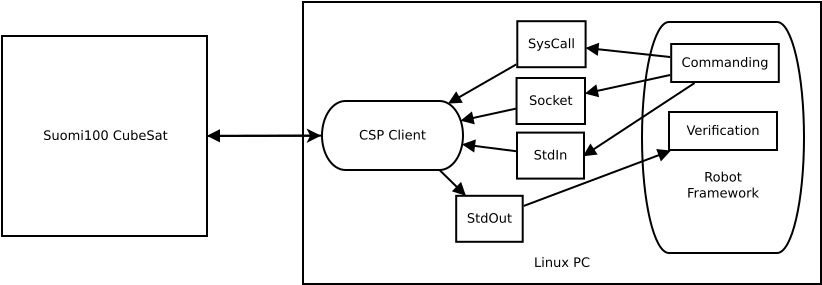
\includegraphics[scale=0.5]{cspautomation}
\end{figure} 
\subsubsection{Python libraries}
In order then to send commands to the client and to automate the testing of the satellite, a set of scripts using \textit{Python} programming language were written, called libraries in the context of Robot Framework. All of these libraries consisted of one Python class each. The class of the core library, known as \textit{CubeSatAutomation}, has the methods to do the communication with the CSP client via any of the three methods, socket, stdin or ? syscall. As well as methods to read and verify the process replies from stdout.
As can be seen in the figure above, the commands are sent to CSP client through any of the three communication routes and the output of the program goes to the standard output or \textit{stdout}. The output is then caught and read by the CubeSatAutomation library and test cases and test steps or keywords are failed or passed based on the output read from the CSP client. \par
Next the test automation libraries are explained in more detail: 
\\
\\
\textbf{CubeSatAutomation library}\par
CubeSatAutomation library has the core functions for sending commands, opening socket connection, opening and closing the opened program and others. Besides being able to open the CSP client program, any program can be automatically opened with the library as the method for opening uses the standard Python \textit{subprocess} library. All the other libraries implemented use the core methods in CubeSatAutomation, for example to send commands to the CSP client to execute. These other libraries have subsystem specific functions for the test automation. To have only one open communication route and one handle on the CSP client program process, the core library defines these as class variables, which are then accessed by the subsystem libraries. This way e.g. only one socket connection is used during an entire Robot Framework test suite and the CSP client is opened and closed only once as well. Another class variable which defines the scope of the instance of the class in the Robot Framework was defined as well. This was chosen to have a value corresponding to the suite level, as the widely used \textit{Selenium2Library} uses the same scope for its class instance in Robot Framework as well. By having the scope on the suite level, only one instance of the library class is declared per test suite, thus again having only one handle on the client software and having only one connection route open during the execution of a test suite.\par 
The essential core methods used in the CubeSatAutomation Python class are explained below:\\
%\textbf{client_start(self, config_file=None, prog=None, params=None)}
\textit{\textbf{Client Start  <config file> <program> <parameters}}\\
Explain.\\
\textit{\textbf{Client Close <socket> <program>}}\\
Explain.\\
\textit{\textbf{Connect Socket <config file> <server> <port>}}\\
Explain.\\
\textit{\textbf{Send Command  <message> <option> <timeout> <read timeout>}}\\
Explain.\\
\textit{\textbf{Write Command  <message> <option> <timeout> <read timeout>}}\\
Explain.\\
\textit{\textbf{Type Command  <message> <option> <timeout> <read timeout>}}\\
Explain.\\
\textit{\textbf{Persistent Command  <message> <exception replies> <end reply> <timeout> <read timeout>}}\\
Explain.\\
\textit{\textbf{Verify Reply Contains  <message> <timeout> <read timeout>}}\\
Explain.\\
\textit{\textbf{Verify Reply Contains Not  <message> <timeout> <read timeout>}}\\
Explain.\\
\textit{\textbf{Verify Reply Contained  <message> <timeout> <read timeout>}}\\
Explain.\\
\textit{\textbf{Wait Until Reply Contains  <message> <timeout> <read timeout>}}\\
Explain.\\
Finally, here are some of the keywords presented that are specific to GomSpace NanoEye.\\
\textit{\textbf{Set Satellite Parameter  <device> <parameter> <value>}}\\
Explain.\\
\textit{\textbf{Send Satellite Parameters}}\\
Explain.\\
Remember to mention that replies can be stored temporarily.\par
Creation of a skeleton core library was the aim of the final development of our test automation library. This library only has the aforementioned methods to start and communicate with a desired Linux program running on terminal shell (or bash shell) and keywords that are more specific to Suomi100 or CSP client were omitted. With the aid of this library, satellite software developers wishing to automate testing of their satellite and satellite software, can then create their own specific libraries suited to their own needs.The final version of the CubeSat test automation library is desribed in section 4.\\
\\
\textbf{Subsystem libraries}\par 
Other libraries developed for test automation of Suomi100 are called \textit{NanoCam.py} and \textit{RadioPayload.py} and these were intended for the automated testing of NanoCam and radio payload subsystems respectively. The classes of both of these create an instance of CubeSatAutomation class instead of calling for specific functions or methods of that class. By doing this the class variables including handle to the automated process, socket address and others are passed to all these other classes as well. The methods of these classes thus use the methods of CubeSatAutomation directly.\par
The specific methods defined by the NanoCam test automation library are presented below as Robot Framework keywords:\\
\textit{\textbf{Camera Startup	<timeout>}}\\
Reboots the camera and downloads parameter table 1 from the subsystem. Timeout specifies the time that we wait for the camera subsystem to come online in satellite bus.\\
\textit{\textbf{Camera Take Picture	<timeout> <store format> <filename> <autogain>}}\\
Sets image format and filename in the camera and takes a picture with the given autogain value (empty at default). Keyword fails if the image is too dark (less 5 \% light) or too bright (over 95 \% light).\\
\textit{\textbf{Camera Load Picture	<stored file> <loaded file>}}\\
Downloads the file stored in NanoCam to the PC running csp-client program.\\
\par
The subsystem specific keywords for the radio payload are defined as the following:\\
\textit{\textbf{Radio Startup  <switch input> <switch power> <antenna input>}}\\
Explain.\\
\textit{\textbf{Radio Powerdown}}\\
Explain.\\
\textit{\textbf{Verify Radio Status}}\\
Explain.\\
\textit{\textbf{Run Radio Mode  <parameter file> <property file> <mode> <mode arguments}}\\
Explain.\\
\textit{\textbf{Verify Radio Results  <buffer file> <timeout>}}\\
Explain.\\
\textit{\textbf{Radio Load Data  <stored file> <loaded file> <timeout>}}\\
Explain.\\
\textit{\textbf{Radio Plot Data  <file> <output file> <plot image>}}\\
Explain.\\
  
 
\begin{itemize}
\item[--]Mention about Robot's Process library, our library has some similar functionality
\item[--]Libraries are Static API version 
%http://robotframework.org/robotframework/latest/RobotFrameworkUserGuide.html#creating-test-libraries 
\end{itemize}     
\subsubsection{Robot framework test suites}
Rewrite this.\par
The test suites follow a keyword-driven approach and the keywords were written to be short and mostly to be non-specific to the test case. In other words, approach was to make smaller set of versatile and generic keywords that could be used over many test cases and test suites. Almost all of the keywords were written purely to the Python libraries. This approach was felt to be more efficient as there would be less need to maintain the test suites if they had large set of specific, though descriptive, keywords. Besides, our satellite project is not a typical software project where stakeholders would go over the test suites and validate them. All people involved in the project have a technical background. In addition, having a set of general keywords that are not entirely tied to our satellit project is beneficial if some future satellite project wishes to use the testing methods and tools described in this thesis.\par 
\subsection{Test setups and environment simulation}
Four different aggregates for testing were identified from Suomi100 satellite and 
for simulating the functional environment of the satellite for these different types of tests, four different environments were arranged(? sopiva sana). Two different environments for testing two different payloads, one for testing basic operational features of the satellite and one larger for the operational scenario testing of the satellite. 
\subsubsection{Environment and setup for camera payload testing}
For the testing of the NanoCam and imaging operation mode, we tried to find something facing the camera with equal colour and brightness values as what the camera would see while in orbit. The easiest solution was to simply take the whole integrated satellite outside on a bright day to the balcony on top of our department in Aalto University.\par 
Below is a Figure N of the test setup used during the testing.\par 
\begin{figure}[h!]
\includegraphics[scale=0.3]{camerabucketspurgu}
\caption{Suomi100 satellite on a balcony during imaging mode tests.}
\end{figure} 
\subsubsection{Environment and setup for radio payload testing}
About simulation done with Hack RF.
\begin{figure}[h!]
\caption{Radio payload testing with hackrf}
\includegraphics[scale=0.3]{payload_testing_hackrf}
\end{figure}
\subsubsection{Environment and setup for satellite basic operations testing}
For testing of the basic satellite operational features like collection of housekeeping and safe rebooting during an error, no external inputs to the satellite were used. The satellite was in our laboratory clean room simply connected to a PC with the CSP-client. 
In Figure N we have a picture of this setup.
\subsubsection{Environment and setup for satellite operational scenario testing}
Solar simulator with a 1800 Watt lamp. Control of the satellite over radio link.
\begin{figure}[h!]
\includegraphics[scale=0.3]{daysetuplamp1}
\caption{Day in the life setup 1}
\end{figure} 
\begin{figure}[h!]
\includegraphics[scale=0.3]{daysetuplink}
\caption{Day in the life setup 2}
\end{figure} 
\begin{itemize}
\item[--]About Suomi100 subsystems
\item[--]About Gomspace software and instrument software
\item[--]Do more traditional functional test suites for different operation modes
and a "day in a life of a satellite" test suite as basis for the acceptance testing comparable to e.g. vibrational testing in importance
\item[--]Operation modes of the satellite, each subsystem has a leading role in each of the operation modes. Operation modes to use cases. From use cases to test suites.
\item[--]Robot framework, acceptance test framework with keywords.
\item[--]Testing environment, gomspace API client
\item[--]Automating control of Suomi100 with Robot and gomspace client. C code added to the gomspace client.
\item[--]Modular python library for automated testing
\item[--]Testing of Camera operation mode, functional tests with different parameters, reboot and crash sequences
\item[--]Testing of radio payload operation modes, functional tests with different parameters, reboot and crash sequences.
Changes made to the code.
\item[--]Testing of communication operation mode and software upload, functional tests with different parameters, reboot and crash sequences
\item[--]Testing the eps with power saving mode, what happens when we run out of power?
\end{itemize}
 

\clearpage

\section{Results and Discussion}
%\section{Tulokset}
\subsection{Executed tests}
The Robot Framework test suites executed can be divided to three categories: test suites done for the two payloads, test suites written for general satellite operations and test suites for "day in the life of the satellite" operational tests. The first category of suites follow more traditional method of combinatioral testing. Yet, each test case was derived from the operation modes defined for the camera and radio payloads. Each of the test cases for their representative operation mode are identical in steps, but use different combination of values in the keyword arguments.\par
The second category consists of test suites made for the functional testing of the commands that contribute to the basic operations of the satellite. Such as telemetry gathering, flight planner commands, software update, etc. In addition, test suite was written for testing restarts of the subsystems and of the OBC and of the whole satellite as well.\par 
The third category, follows the higher level satellite integration tests where we test the satellite based on operational scenarios. Separate test suites were written for each operational scenario.\par
In addition to these test suites, another one was used during the development of the software for the radio payload. This test suite resembles a smoke test and it has limited set of test cases, testing each of the operation modes. Yet, no proper continous integration chain was done during this time, but the smoke tests were manually started usually once every week.\par   
\subsubsection{Tests for camera payload}
The test cases for the NanoCam were identical in structure, or in other words, we made several test cases for the same use case of the camera payload. Only difference was that the main parameters like gain value and exposure time differed between test cases. These two are the main parameters according to the NanoCam manual provided GomSpace. Having the exposure time fixed, we demonstrated the use of combinatorial testing to go through different variations of the camera parameters. Three different values of the exposure time were used and for each value, the same parameters other than exposure time were changed in different test cases. The values used for the exposure time were ${10 000 \mu s}$, ${30 000 \mu s}$ and ${90 000 \mu s}$.  Below is a Figure N showing the test case structure used in testing of the camera payload.\par
\begin{figure}[h!]
\includegraphics[scale=0.5]{cameracase}
\caption{Robot Framework test case structure for camera payload testing.}
\end{figure}
As can be seen from the example test case, the test covers such features as NanoCam restart and detection in the satellite bus, the use of different camera parameters and finally, image taking, storing and transfer from the satellite. All the taken images where then added to the Robot Framework log files, which gives a comprehensive view on how the different camera parameter values affected the taken images.\par 
For the environment simulation, the attempt was to find a really sunny day to give some indication of the brightness of the pictures while the satellite is in orbit. This was achieved to some extent, but at the start of the test few clouds appeared and some pictures turned out very bright and some less so. If the level of light would have stayed the same during the whole test, we could have gotten some baseline idea on the affects of the different parameters on the images.\par
Nonetheless, no test cases failed due to software errors. Thus, we gotten some confidence that changing different parameters didn't crash the software or that any combination of parameters didn't cause problems in the functioning of the satellite. We saw as well that the images didn't become distorted in any way. Out of the 39 test cases, 9 failed because the light level was too high. Yet, the brightness in space around Earth is much higher than what we can have here on the surface even at the brightest day [source], not to mention the fact that the tests were conducted in Finland. Thus, increasing the exposure time or gain value while in orbit will make the images to be too bright and so, setting the camera parameters to their default values would possibly give us the best pictures. On another note, the automation of these tests was the first time our automation libraries along with Robot Framework were used to properly test Suomi100 satellite and thus these tests worked as a technology demonstration as well. Below are some pictures taken with the camera.\par
Most importantly, the tests demonstrated that the integration with the rest of the satellite was succesful. As in fact, there was a defect in the integration of the camera with the satellite at the first time the satellite platform arrived to us. The camera lense was too far away from the cell in the PCB of the camera subsystem and the first test pictures taken with the camera were distorted. The manufacturer of the satellite platform provided us with a test picture that the camera was working properly, but it seems that they didn't test the camera after it was integrated to the satellite. After this problem was found, GomSpace provided us with a new camera and the integration of this worked properly. The Robot Framework tests worked thus also as the verification tests for the integration of the NanoCam subsystem to the satellite platform.\par 
\begin{figure}[h!]
\includegraphics[scale=0.2]{def}
\caption{Picture taken with default parameters from NanoCam manual.}
\end{figure}
\begin{figure}[h!]
\includegraphics[scale=0.2]{def23}
\caption{Picture taken with exposure time 30 000 microseconds and without gamma correction.}
\end{figure}
\subsubsection{Tests for radio payload}
During the development of the software for the payload radio, a small test suite was used for smoke testing of the software and the payload. Basically, the test cases tested that the commands are executed without errors and that the radio can output data. This test suite was also used when the payload was integrated to the satellite.\par
The three tests in this suite were run at least once a week during the development of the software, but a proper \textit{Continuous Integration/Continuous Development} pipeline was not used where for example flashing of a new software to the NanoMind would have caused these test to run automatically.\par
Besides the aforementioned smoke tests, a more comprehensive set of test suites was performed for the radio payload after it was confidently integrated to the satellite platform. As the hardware and software were of our own design and the integration happened with a platform manufactured by another organization, these tests took the most time of all automated tests done on Suomi100 satellite. A few sessions were held where we ran these comprehensive test suites for the radio payload and each time new defects in the code and in the integration were found. Of all the tasks related to Suomi100, the proper integration of the radio payload to the GomSpace 1U NanoEye took the most effort from us.\par
Test cases for our payload followed the combinatorial testing method in a way where all the the test suites for a given radio operation mode had the same test cases but the frequency used was different. In addition, the test suites for different radio operation modes differed as each had a bit different parameters. These test suites then covered some amount of different parameter combinations and as with the camera payload, the measurement data was downloaded from the satellite and then processed and plotted and the plot images were added to the Robot Framework HTML log files.\par 
Below is an example of the test case structure used in testing of the radio payload.\par 
\begin{figure}[h!]
\includegraphics[scale=0.5]{payloadrfwtest}
\caption{Robot Framework test case structure for radio payload testing.}
\end{figure}
Most interesting information about the payload operation was found from the csp-client replies outputted to the log files, as what we were measuring was static and as such nothing too much could have been said about the test cases just by looking the measurement plots. Besides that the values were not zero or that there was actual variance in the values measured. In Figure N below we have one plot produced from measurement made with the radio while the satellite was at our laboratory facility and no external radio signal sources were used from our part.\par 
\begin{figure}[h!]
\includegraphics[scale=0.6]{m1_debug1}
\caption{Plot of measurements of radio static made by the radio payload at 5 Mhz.}
\end{figure}
About the emergent problems with the integration with NanoMind which ultimately led us to drop the sample rate to 1 Khz. FreeRTOS tasks, developed with raspi 3 etc. Antcap value was zero/one in all cases->a function was made to calculate it. Problems with the GPIO pins, only three were functional while 6 were needed.     
\subsubsection{Tests for basic satellite operations}
Testing of the basic functionalities of the satellite software was felt to be necessary. Thus, tests were performed for satellite features such as safe satellite reboots, different housekeeping commands, flight planner commands and flight software updating. All of these can be seen as the basic functionalities which all of the other operations of the satellite depend upon. Test suites for these features don't follow the combinatorial testing methods used for two payload subsystems. Instead, test cases are based on different use cases or different situations we might end up facing with the satellite. In addition, the keywords used were less subsystem specific and more of the test cases used the generic keywords, such as \textit{Send Command} and \textit{Verify Reply Contained}.\par
\textbf{Reboot tests}
\par 
Twelve test cases were written for satellite reboots during different situations. The goal of these tests was to find out if during some operation, e.g. file upload, we can get the NanoMind stuck so that it doesn't reboot safely anymore. This test suite also has test cases simply to shutdown different subsystems and to verify their absence in the satellite bus with the simple \textit{ping} command. From these test cases, it was found that the NanoCom communication system couldn't be shutdown completely. It still replied to ping commands even though a command was sent to shut it down. This functionality naturally is preferable (NanoCom manuaali sanoo tästä jotain?) and though this led to one test case of the reboot test suite to fail, the test can be seen to fail positively. As such, 11 test cases passed and one failed positively from this test suite. \par
The other types of test cases in the reboot test suite tested reboots during satellite operations and the reboots were mostly caused by adding reboot commands to the flight planner so that they would occur during some satellite operation, e.g. during radio payload operation. In all of these, the satellite came back safely. Yet, it has been several times that the NanoMind can get stuck and in those situations to get the OBC working again, it has required us to either manually reboot the EPS or to send a command via another subsystem to reboot the NanoMind. The satellite has recovered safely from these situations after reboot. But when we are using the satellite control software, csp-client, we are not able to do this. Which raises a few eyebrows whether there can happen something during orbit that causes the satellite to be stuck forever.\par
Fortunately, there are several watchdogs in the satellite that in theory can trigger a reboot after a certain time. Unfortunately, we were not able to deliberately trigger a situation where NanoMind is stuck and thus tests for these watchdog functionalities had to be omitted from the test suite.\par 
\textbf{Housekeeping tests}
\par 
Another 11 test cases were performed to test the housekeeping features provided by the GomSpace platform. Test cases were written for different housekeeping commands of different subsystems as well as for housekeeping data storing and transfer from the satellite. Testing of the beacon functionality was as well included in this test suite, as the beacon outputs recent HK information. Plotting of the beacon data was developed during the realization of these tests by another member of the satellite team, Petri Koskimaa, and by the thesis author. These plotting functionalities were later used in the "day in the life of the satellite"-tests as well. All test cases of this test suite passed without errors. Meaning, all the commands did what they were supposed to do. Which, obviously is the preferred result. In Figure N we have an example picture of a plot of the system current provided by the beacon at different timestamps.\par 
\begin{figure}[h!]
\includegraphics[scale=0.6]{hk_plot_cam_op2}
\caption{System current from the beacon data during imaging mode operation mode.}
\end{figure}
\textbf{Flight planner tests}
\par 
For testing of the flight planner feature, seven test cases were performed. The feature was tested with some basic flight planner creation commands as well as with more complicated ones. Out of all these tests involving basic functionalities of our satellite, this one had the most failed test cases. For first, it was assumed that giving the commands in wrong format (string instead of an integer) would cause the csp-client to indicate an error. Yet, such a thing didn't happen but giving the commands in wrong format didn't cause the software to crash either. In addition, if the command string was too long, an error was indicated and no flight planner command was appended to flight plan list. Which happened to be the case when we tried to give one specific command for our radio payload, but this command to run the radio payload in one of the defined operation modes happens to be the single most essential command for the payload! Thus, in order to make it work with the flight planner we need to modify the source code for the flight planner so that it can accept longer strings as commands (ei tehty vielä!). Otherwise, we can only use the radio payload when the satellite is in the reach of our communication radios. Which isn't preferrable as we would be radically limiting the area what we can measure.\par
\textbf{Software update tests}
\par 
Three test cases were performed for the software update feature. These test cases took a longer time to run than the other test cases involving the basic functionalities of the satellite. Naturally so, as we had to upload the new software to the satellite via the USB on the NanoUtil. These tests tested basic uploading of a new software image, rebooting back to the software that was flashed to NanoMind and tested uploading of an invalid file as an image to the new software. The satellite passed all these tests as expected, thus we have some confirmation that we actually can upload a new software to the satellite and tell it to reboot using that.\par
In the test case where we uploaded and invalid file as an image, the file itself was just a binary file containing measurement values from the payload radio. Booting with this file caused the NanoMind to crash with EXCEPTION 13 error message. Also, we had set the NanoMind to try to boot with this file three times and it crashed each time with this error, but eventually as the boot counter reached zero, the satellite managed to recover the proper software it was flashed with. Which gave us good knowledge that the satellite manages to recover itself if we happen to upload a software to the satellite that causes unexpected reboots.\par     
\subsubsection{Tests for operational scenarios of the satellite}
Test suites were formed to test different phases of the scenarios that the satellite will encounter while in orbit. A scenario would be e.g. where we come from the eclipse, send commands to the satellite and downlink data. Each step in the scenario, like downlinking of data, formed its own test case within the test suite.
\subsection{Release version of CubeSatAutomation test library}
Cleaned of Suomi100 dependencies. Present keywords etc. 
\subsection{Developing operational scenario tests as requirement for CubeSat mission readiness}
Vibrational tests are required. Could higher level functional tests like the "day in the life of the satellite" operational scenario tests be pushed as another requirement for mission readiness. A guarantee that the satellite is ready for launch into space. Similar to testing for mission readiness at this level done by NASA and others, but "simpler"?\par 
What kind of documentation? Is it affordable for all CubeSat teams? Maybe the testing methods developed here can be utilized, like the python libraries with Robot Framework?\par
\subsection{Further lessons learned from testing of Suomi100 CubeSat}
More rigorous requirement specifications, they would help higher level functional testing.
What it should do, what it shouldn't do. Some area of operation, etc. More rigorous identification of operational scenarios and operation modes. All these in the vein of the CubeSat concept, not too rigorous or too formal, yet covering all the situations. Some examples from industry or other CubeSat missions?\par  
\begin{itemize}
\item[--]Summary of the work done and were the goals accomplished?
\item[--]Summary of test results
\item[--]How operation modes behaved during tests
\item[--]How the different subsystems behaved during tests
\item[--]How the instrument behaved during tests
\item[--]Importantly: What issues with the software and subsystems were found with the tests and what corrections were implemented based on the test results
\item[--]AFTER LAUNCH ???:
\item[--]Operation modes
\item[--]Things that worked, commands that went through
\item[--]About failures if those happened, software crashes
\item[--]Did we manage to prevent failures that were pointed out as the common causes in Cubesat failure database and in research done by Swartwout?
\item[--]What was found during testing and comparison to how the satellite performed in orbit. Did the implemented changes to the software improve reliability.
\end{itemize}


%% Huomaa seuraavassa kappaleessa lainausmerkkien ulkopuolella piste, 
%% koska piste ei lopeta lainattua tekstinp\"atk\"a\"a.
%% Jos lainattu tekstinp\"atk\"a loppuu v\"alimerkkiin, tulee v\"alimerkki
%% lainausmerkkien sis\"alle: 
%% "Et tu, Brute?" sanoi Caesar kuollessaan.


\clearpage

\section{Conclusions} 
%\section{Yhteenveto}
In this thesis automated functional system integration tests for Suomi100 CubeSat were performed with Robot Framework. The need for testing at this level was identified from surveys conducted for all CubeSat missions flown previously, which showed a high failure rate for University led missions in contrast to low failure rates for missions performed by organisations and companies with established practices in integration and testing. Thus, testing methods used by e.g. NASA at satellite integration level along with industry proven testing practices were applied in design of testing performed for Suomi100. The testing was automated with Robot Framework, which is an industry proven acceptance testing framework. It was felt that doing the testing with the help of an automated computer software would give the testing more rigour and reproducibility. For automating the control of the satellite in interest of test automation, libraries for use with Robot Framework were programmed with Python programming language.\par
First tests conducted for the satellite were functional tests for integrated Suomi100 payloads, which are an optical camera and a radio instrument for ionospheric measurements. Second test set included acceptance testing of the core satellite functions  such as housekeeping data collection, safe reboot handling, software updates and so forth. Final set consisted of tests for operational mission scenarios or "day in the life of the satellite"-tests.\par 
An attempt was made with our limited resources to simulate the functional environment for testing of the payloads as well as for the operational scenario tests. For testing of the camera payload, the satellite was taken to a balcony at our department on a sunny day. During the testing of the integrated radio payload,  a HackRF software defined radio was used to simulate the noise signals found in the ionosphere. A larger setup was used for the "day in the life of the satellite"-tests. With this test, we tested not just the proper functionality of the satellite software but that the radio link to the satellite works and that the solar panels can charge the satellite. Thus, the automated tests were performed via the radio link and a large Xenon lamp was used to simulate the Sun.\par 
With the performed tests, we proved proper functionality of the camera payload as well as proper functionality for almost all of the tests conducted for the core satellite functions.   The operational scenario tests showed that we can communicate with and send commands to the satellite via radio link and that the solar panels can charge the batteries in Suomi100. Only downside seemed to be the low downlink speed, yet this was to be expected.\par 
The tests for the radio payload on the other hand presented several defects and most importantly emergent problems in the integration with the rest of the satellite platform. The defects were fixed with consequent software updates, but certain problems with integration couldn't be overcome. The biggest one being the slow speed of reading and storing of data from the payload by the OBC. This forced us to drop the sample rate from the possible 32-48 kHz to just 1 kHz for reliable data measurement.\par  
Performing of these tests proved to us that Robot Framework can work as a testing framework for CubeSats and that we could carry out automated testing of Suomi100 CubeSat. The software libraries doing the actual automation were developed into a generic testing library, which potentially could be used for testing and automation of any Linux terminal software, such as a satellite ground station control software.\par 

\begin{itemize}
\item[--]Did we improve the functionality and reliability of the satellite?
\end{itemize}



\clearpage
%% L\"ahdeluettelo
%%
%% \phantomsection varmistaa, ett\"a hyperref-paketti latoo hypertekstilinkit
%% oikein.
%%
%% The \phantomsection command is nessesary for hyperref to jump to the 
%% correct page, in other words it puts a hyper marker on the page.

\phantomsection
\addcontentsline{toc}{section}{\refname}
%\addcontentsline{toc}{section}{References}
\begin{thebibliography}{99}

%% Alla pilkun j\"alkeen on pakotettu oikea v\"ali \<v\"alily\"onti>-merkeill\"a.
\bibitem{Swart1} Swartwout, Michael\\
  \textit{The First One Hundred CubeSats: A Statistical Look}, Journal of small satellites, 2013.
\bibitem{sularikurssi} Laplante, Phillip A. \& Ovaska Seppo J.\\
  \textit{Real-Time Systems Design and Analysis}, 4th edition, IEEE Press, USA 2012.
\bibitem{testingcomplex} Pries, Kim H. \& Quigley Jon M.\\
  \textit{Testing Complex and Embedded Systems}, Taylor and Francis group, CRC Press, USA 2011.  
\bibitem{Swart2016} Swartwout, Michael\\
  \textit{Secondary Spacecraft in 2016: Why Some Succeed (And Too Many Do Not)}, Some IEEE publication, 2015.
\bibitem{SpaceWorks2017} Doncaster, Bill \& Williams Caleb \& Shulman Jordan\\
  \textit{2017 Nano/Microsatellite Market Forecast}, Some IEEE publication, 2015.

\bibitem{Swart2015} Swartwout, Michael\\
  \textit{Secondary Spacecraft in 2015: Analyzing Success and Failure}, Some IEEE publication, 2015.
\bibitem{Langer} Langer, Martin \& Bouwmeester Jasper\\
  \textit{Reliability of CubeSats - Statistical Data, Developer's Beliefs and the Way Forward}, 30th Annual AIAA/USU Conference on Small Satellites, 2016.
\bibitem{smallsatconf31}
  \textit{http://spacenews.com/cubesat-reliability-a-growing-issue-as-industry-matures/}, obtained 12th of December, 2017.  
\bibitem{ssvi}
  \textit{https://www.nasa.gov/smallsat-institute}, obtained 12th of December, 2017. 
\bibitem{Jacklin} Jacklin, Stephen A.\\
  \textit{Survey of Verification and Validation Techniques for Small Satellite Software Development}, Space Tech Expo Conference USA, CA, 2015.
\bibitem{robotmain}
  \textit{http://robotframework.org/}, obtained 28th of January 2018.
\bibitem{klerkdippa} Laukkanen, Pekka\\
  \textit{Data-Driven and Keyword-Driven Test Automation Frameworks}, Helsinki University of Technology, 2006.  


\end{thebibliography}

%% Appendices
%% Liitteet
\clearpage

\thesisappendix

\section{Esimerkki liitteest\"a\label{LiiteA}}
\begin{lstlisting}[language=C]
/*
Radio Operation modes
*/
#include <radio.h>

#include <inttypes.h>
#include <string.h>
#include <stdio.h>
#include <stdint.h>
#include <string.h>
#include <ctype.h>
#include <stdlib.h>
#include <pthread.h>
#ifdef linux
#include <time.h>
#else
#include <FreeRTOS.h>
#include <task.h>
#endif

#include <util/console.h>
#include <util/log.h>
#include <util/color_printf.h>
#include <util/clock.h>

#include <csp/csp.h>
#include <csp/csp_endian.h>
#include <csp/arch/csp_thread.h>
#include "radio_config.h"
#include "libradio.h"
#include "radio_calculation.h"
#include "radio_property.h"


// Syntax for different arguments val1;val2;val3; 
// NOTE: Frequency in kilohertz
void raw_data_mode(char *mode_args)
{
	uint32_t t_start = 0;
	uint16_t f_const = 0; 
	uint32_t n_times = 0;
	uint32_t t_sleep = 0;
	uint8_t ferrite = 0;
	char temp[32] = {0};
	unsigned int i = 0;
	unsigned int j = 0;
	unsigned int argc = 0;
	while(i < strlen(mode_args))
	{
		if(mode_args[i] != ';')
		{
			temp[j] = mode_args[i];
			j++;
		}
		else
		{
			if(argc == 0)
				t_start = strtol(temp, NULL, 10);
			else if(argc == 1)
				f_const = strtol(temp, NULL, 10);
			else if(argc == 2)
				t_sleep = strtol(temp, NULL, 10);
			else if(argc == 3)
				n_times = strtol(temp, NULL, 10);
			else if(argc == 4)
				ferrite = strtol(temp, NULL, 10);
			j = 0;
			argc++;
			printf("temp:%s\n", temp);
			memset(temp, 0 ,sizeof(temp));
			if(argc > 4)
				break;
		}
		printf("%c", mode_args[i]);
		i++;
	}
	printf("Arguments received for operation:%d %d %d %d %d\n", t_start, f_const, t_sleep, n_times, ferrite);
	// If values invalid for some reason, use these default values
	if(t_start < 0)
		t_start = 0;
	if(f_const < 149 || f_const > 50000)
		f_const = 5000;
	if(t_sleep < 1)
		t_sleep = 100;
	if(n_times < 1)
		n_times = 100000;
	if(ferrite < 0 || ferrite > 1)
		ferrite = 0;
	printf("Arguments corrected for operation:%d %d %d %d %d\n", t_start, f_const, t_sleep, n_times, ferrite);
	// sleep or vTaskDelay
	#ifdef linux
		usleep(t_start*10);
	#else
		vTaskDelay(t_start);
	#endif
	printf("Radio raw data mode commencing\n");
	//Choose ferrite with the switch command, how?
	
	// Open file for appending/writing
	// in FreeRTOS create file in /flash/...

	// Read from spi
	#ifdef linux
		uint32_t start_time = 0;
		uint32_t end_time = 0;
	#else
		timestamp_t *start_time = malloc(sizeof(timestamp_t));
		timestamp_t *end_time = malloc(sizeof(timestamp_t));
	#endif

	#ifdef linux
		start_time = (int)time(NULL);
	#else
		clock_get_time(start_time);
	#endif
	uint16_t *data = calloc(10, sizeof(int));
	FILE *dfp;
	// Get system time to the filename, FreeRTOS has some command ?
	char filename[64] = {0};
	char filetime[64] = {0};
	#ifdef linux
		sprintf(filetime, "%d", (int)time(NULL));
	#else
		sprintf(filetime, "%d", start_time->tv_sec);
	#endif	
	strcat(filename, "m1_");
	strcat(filename, filetime);
	strcat(filename, ".csv");
	if((dfp = fopen(filename, "a")) == NULL)
		fprintf(stderr, "Could not open %s\n", filename);
	fprintf(dfp, "Val,Freq\n");

	// si chip takes frequency in khz
	radio_am_tune_freq("0", f_const, 0);
	// Wait for chip stabilization
	#ifdef linux
		usleep(t_sleep*10);	// usleep is deprecated in POSIX, nanotime is preferred
	#else
		vTaskDelay(t_sleep);	// Milliseconds
	#endif
	for(unsigned int n = 0; n < n_times; n++)
	{
		//spi_16read(data);
		 
		// Append to file
		fprintf(dfp, "%d,%d\n", n, f_const);	
	}
	#ifdef linux
		end_time = (int)time(NULL);
		fprintf(dfp, "\nStart: %d End: %d\n", start_time, end_time);	
	#else
		clock_get_time(end_time);
		fprintf(dfp, "\nStart: %d End: %d\n", start_time->tv_sec, end_time->tv_sec);	
		free(start_time);
		free(end_time);
	#endif	

	fclose(dfp);	
	free(data);
} 
\end{lstlisting}



\clearpage
\section{Toinen esimerkki liitteest\"a\label{LiiteB}}
\begin{lstlisting}
*** Settings ***
Library		libclient.py
Suite Teardown	Client Close	${sock}		{proc}

*** Test Cases ***

Test Setup
	${proc}=		Client Start	/home/juha/S100/EGSE/EGSE/csp-client-v1.1/build/csp-client	-a 8 -d /dev/ttyUSB0 -b 500000
	#${proc}=		Client Start	/home/juha/S100/EGSE/EGSE/csp-client-v1.1/build/csp-client	-a 10 -z localhost
	Set Suite Variable	${proc}
	Sleep			5
	${sock}=		Connect Socket	s100-juha	5000
	Set Suite Variable	${sock}


Target Mode
	[Documentation]		The payload radio performs several sweeps over the entire frequency range.
	[Tags]			OPMODE-TARGET
	Store Client Responses	${proc}	 Target Mode
	# Are we sure that we start the thread in the satellite?
	#Run Radio Mode		${sock}  ${proc}  /home/juha/S100/confs/radio_params.cfg  /home/juha/S100/confs/radio_props.cfg  3  0;0;0;0;0;0;0;0;0;
	Run Radio Mode		${sock}  ${proc}  /flash/radio_params.cfg  /flash/radio_props.cfg  3  0;0;0;0;0;0;0;0;0;
	Sleep			2
	# Add proper hk and beacon commands here with flight planner
	# csp-client doesnt have flight planner
	#Get HK			${sock}		${proc}		30
	#Send Beacon		${sock}		${proc}		10	
	Verify Radio Results	Target Mode
	Send Message		${sock}		${proc}		exit_client
	Close Connection	${sock}

\end{lstlisting}


\end{document}
